


\documentclass[a4paper,12pt,spanish]{article}

\usepackage[utf8]{inputenc}


\usepackage{blindtext}
%\usepackage{microtype}
\usepackage{amsfonts, amsmath, amsthm, amssymb}
%\usepackage{fancyhdr}
%\usepackage{index}
%\usepackage{multicol}    

\usepackage[T1]{fontenc}
\usepackage[utf8]{inputenc}
\usepackage{graphicx}
\usepackage[spanish,es-tabla]{babel}
\usepackage{url}
\usepackage{enumitem}

\usepackage[unicode=true, pdfusetitle,
bookmarks=true,bookmarksnumbered=false,bookmarksopen=false,
breaklinks=true,pdfborder={0 0 1},backref=false,colorlinks=false]
{hyperref}

\usepackage{listings}


\usepackage{siunitx} %para el sistema internacional
\usepackage[export]{adjustbox}
\usepackage{booktabs} 
\usepackage{subcaption}

\usepackage{float}


\newcommand{\address}[1]{
	\par {\raggedright #1
		\vspace{1.4em}
		\noindent\par}
}


\pagenumbering{gobble}
\include{noNumberPage}
\pagenumbering{arabic}
\setcounter{page}{37}

%tutorial de tablas latex: https://manualdelatex.com/tutoriales/tablas

\usepackage{multirow}

% \usepackage[table,xcdraw]{xcolor}


%Inicio del documento (hasta que se cierre con \end{document}
\begin{document}
	
	
	\title{Distribución de campo magnético de una bobina plana}
	
	%\author{Adrián Rivero Fernández}
	\date{}
	
	\maketitle
	
	
	
	\begin{abstract} %resumen
		
		En esta práctica mediremos los campos magnéticos creados por bobinas. 
		
		Estudiaremos el campo creado por una bobina casi plana y el correspondiente a dos bobinas iguales dispuestas coaxialmente. Verificaremos si se cumple la condición de Helmholtz de las bobinas: que la mínima variación del campo sobre la zona central del eje entre bobinas se produce cuando la distancia entre estas es igual a su radio.
		
	\end{abstract}

\section{Introducción}

El campo magnético creado por una espira circular de radio $a$ a lo largo del eje se obtiene mediante la ley de Biot y Savart:
\[B = \frac{\mu_0 i a^2}{2(a^2 + z^2)^{3/2}} u_z\]
siendo i la corriente que circula por la espira. 

Para $N$ espiras alrededor de una circunferencia de radio $a$, la expresión sería:
\[B = N\frac{\mu_0 i a^2}{2(a^2 + z^2)^{3/2}} u_z\]

Para $z= 0$, en el centro de la espira, tenemos
\[B = \frac{\mu_0 N_i}{2a}u_z\]

Para un campo creado por una corriente continua, podemos detectar el campo con una sonda basada en el efecto Hall. Para un campo creado por corriente alterna, se detecta con una pequeña bobina de prueba (20 mH), de modo que perturbe lo mínimo la distribución de campo, y su radio sea unas 20 veces menor al de la bobina que genera el campo.

La fuerza electromotriz inducida en la bobina de prueba, siendo $B = B_0 \cos \omega t$, es: 
\[ \mathcal{E} = -\frac{d \phi}{dt} = \omega B_0 K \sin \omega t\]

siendo $\omega = 2\pi f$, $K$ la constante de la bobina y $B_0$ la amplitud de campo magnético creado por la bobina circular al aplicar la corriente $i = I_0 \cos(\omega t)$.
Suponiendo que la dirección y sentido de $B_0$ es el mismo del vector normal a la sección de la bobina de prueba.
En caso contrario, se manifestará el coseno del angulo entre ellos en la expresión para el campo B.

En el centro de la espira tenemos entonces:
\[ \mathcal{E} = K \cdot \frac{\mu_0 N I_0}{2a} \omega \sin \omega t\]

A partir de esta expresión puede ser representada por una recta de pendiente
\[C= K \frac{\mu_0 \omega N}{2 a }\]

de la que podemos calcular la constante $K$ de la bobina de prueba, y a partir de ahí determinar la amplitud del campo magnético, $B_0$


\section{Material y Métodos}


Nuestro dispositivo experimental consta de dos bobinas de unos 16cm de radio $a$ y $N = 400$ espiras, colocados sobre un soporte de metacrilato, de modo que se encuentren enfrentadas, y a una distancia medible con una regla sobre la mesa, y ajustable.

Disponemos de una bobina de prueba de unos 20mH y 0,5cm de radio.

Tenemos un osciloscopio, un oscilador de baja frecuencia para que suministre el voltaje a las bobinas, una resistencia patrón de 150 $\si{\ohm}$.


\begin{figure}[H]
	\centering
	\includegraphics[width=1\linewidth]{"../fotos/WhatsApp Image 2022-06-14 at 8.07.03 PM"}
	\caption{}
	\label{fig:whatsapp-image-2022-06-14-at-8}
\end{figure}

Realizaremos tres pruebas diferentes:

\subsection{Calibración de la bobina de prueba}

Situaremos una bobina casi plana sobre su soporte, y conectaremos la fuente de alimentación y la resistencia patrón.

Mediremos la tensión en bornes de la resistencia patrón en el canal 1 del osciloscopio, determinando la corriente que circula por la bobina.

Luego mediremos la tensión inducida en la bobina de prueba, conectada al canal 2 del osciloscopio. Comprobamos que la tensión inducida es máxima cuando el campo es perpendicular a la sección de la bobina de prueba. Realizamos esto con tres frecuencias distintas: 1kHz, 5kHz y 7,5kHz.

A partir de estos datos, representamos gráficamente el voltaje en función de la corriente suministrada, para cada frecuencia, obteniendo la pendiente $C$:
\[C = K\frac{\mu_0 \omega N}{2a}\]

Obtenemos la constante $K$, con lo que podemos calcular la amplitud del campo magnético creado.

\subsection{Distribución del campo creado por una bobina}

Mediremos la intensidad magnética en función de las tres coordenadas cilíndricas $r$, $\varphi$ y $z$.

Sebre la bobina casi plana, con la bobina de prueba paralela al plano de la otra bobina, fijamos un valor de $\varphi$ y tomamos medidas en distintos valores de $r$. De forma similar, fijamos un $r$ y tomamos medidas para distintos angulos $\varphi$. Por último, para un mismo $r$ y $\varphi$, medimos a distintas distancias $z$.

Estos valores del campo los representamos gráficamente en función de las coordenadas cilíndricas.

\subsection{Distribución del campo creado por dos bobinas dispuestas coaxialmente. Bobinas de Helmholtz}

Colocamos en el soporte ambas bobinas planas idénticas, y las conectamos al generador de modo que los campos generados tengan la misma dirección y sentido. Ambas bobinas deben estar alineadas, de modo que tengan el mismo eje central.

Mediremos la distribución del campo sobre el eje para tres distancias diferentes de las bobinas: menor a su radio, igual y mayor. De este modo podremos comprobar si se verifica la condición de Helmholtz.



\section{Resultados y discusión}


\subsection{Calibración de la bobina de prueba}

Hemos tomado los datos en la Tabla 1, y representado el voltaje inducido en función de la intensidad en las Figuras 2, 3 y 4.
En la Tabla 2 recogemos los valores calculados para C y K.

\begin{table}[H]
	\centering
	\begin{tabular}{|lllll|}
		\hline
		\multicolumn{5}{|c|}{f (Hz) = 1000}                                                                                                                                                 \\ \hline
		\multicolumn{1}{|l|}{\begin{tabular}[c]{@{}l@{}}Pos.\\ amplitud\end{tabular}} & \multicolumn{1}{l|}{$V_{fuente}(\si{V})$} & \multicolumn{1}{l|}{$V_R(\si{V})$}    & \multicolumn{1}{l|}{$V_{ind}(\si{V})$}   & $I_R(\si{A})$      \\ \hline
		\multicolumn{1}{|l|}{1}                                                       & \multicolumn{1}{l|}{6}         & \multicolumn{1}{l|}{0,52 $\pm 0,02$}  & \multicolumn{1}{l|}{0,07$\pm 0,02$}   & 0,0035$\pm 0,0001$  \\ \hline
		\multicolumn{1}{|l|}{2}                                                       & \multicolumn{1}{l|}{7}         & \multicolumn{1}{l|}{0,62 $\pm 0,02$}  & \multicolumn{1}{l|}{0,085$\pm 0,05$}  & 0,0042 $\pm 0,0001$ \\ \hline
		\multicolumn{1}{|l|}{3}                                                       & \multicolumn{1}{l|}{8}         & \multicolumn{1}{l|}{0,72 $\pm 0,02$}  & \multicolumn{1}{l|}{0,095$\pm 0,05$}  & 0,0048$\pm 0,0001$  \\ \hline
		\multicolumn{1}{|l|}{4}                                                       & \multicolumn{1}{l|}{9}         & \multicolumn{1}{l|}{0,8 $\pm 0,05$}   & \multicolumn{1}{l|}{0,1075$\pm 0,05$} & 0,0053$\pm 0,0001$  \\ \hline\hline
		\multicolumn{5}{|c|}{f (Hz) = 5000}                                                                                                                                                 \\ \hline
		\multicolumn{1}{|l|}{\begin{tabular}[c]{@{}l@{}}Pos.\\ amplitud\end{tabular}} & \multicolumn{1}{l|}{$V_{fuente}(\si{V})$} & \multicolumn{1}{l|}{$V_R(\si{V})$}    & \multicolumn{1}{l|}{$V_{ind}(\si{V})$}   & $I_R(\si{A})$      \\ \hline
		\multicolumn{1}{|l|}{1}                                                       & \multicolumn{1}{l|}{6}         & \multicolumn{1}{l|}{0,11$\pm 0,01$}  & \multicolumn{1}{l|}{0,0675$\pm 0,05$} & 0,00073$\pm 0,00007$ \\ \hline
		\multicolumn{1}{|l|}{2}                                                       & \multicolumn{1}{l|}{7}         & \multicolumn{1}{l|}{0,125$\pm 0,01$} & \multicolumn{1}{l|}{0,085$\pm 0,05$}  & 0,00083$\pm 0,00007$ \\ \hline
		\multicolumn{1}{|l|}{3}                                                       & \multicolumn{1}{l|}{8}         & \multicolumn{1}{l|}{0,145$\pm 0,01$} & \multicolumn{1}{l|}{0,095$\pm 0,05$}  & 0,00096$\pm 0,00007$ \\ \hline
		\multicolumn{1}{|l|}{4}                                                       & \multicolumn{1}{l|}{9}         & \multicolumn{1}{l|}{0,165$\pm 0,01$} & \multicolumn{1}{l|}{0,105$\pm 0,05$}  & 0,00110$\pm 0,00007$ \\ \hline\hline
		\multicolumn{5}{|c|}{f (Hz) = 7500}                                                                                                                                                 \\ \hline
		\multicolumn{1}{|l|}{\begin{tabular}[c]{@{}l@{}}Pos.\\ amplitud\end{tabular}} & \multicolumn{1}{l|}{$V_{fuente}(\si{V})$} & \multicolumn{1}{l|}{$V_R(\si{V})$}    & \multicolumn{1}{l|}{$V_{ind}(\si{V})$}   & $I_R(\si{A})$      \\ \hline
		\multicolumn{1}{|l|}{1}                                                       & \multicolumn{1}{l|}{6}         & \multicolumn{1}{l|}{0,065$\pm 0,01$} & \multicolumn{1}{l|}{0,08$\pm 0,05$}   & 0,00043$\pm 0,00007$ \\ \hline
		\multicolumn{1}{|l|}{2}                                                       & \multicolumn{1}{l|}{7}         & \multicolumn{1}{l|}{0,08$\pm 0,01$}  & \multicolumn{1}{l|}{0,095$\pm 0,05$}  & 0,00053$\pm 0,00007$ \\ \hline
		\multicolumn{1}{|l|}{3}                                                       & \multicolumn{1}{l|}{8}         & \multicolumn{1}{l|}{0,09$\pm 0,01$}  & \multicolumn{1}{l|}{0,11$\pm 0,05$}   & 0,0006$\pm 0,00007$  \\ \hline
		\multicolumn{1}{|l|}{4}                                                       & \multicolumn{1}{l|}{9}         & \multicolumn{1}{l|}{0,1$\pm 0,01$}   & \multicolumn{1}{l|}{0,1225$\pm 0,05$} & 0,00067$\pm 0,00007$ \\ \hline
	\end{tabular}
	\caption{}
\end{table}



\begin{figure}[H]
	\centering
	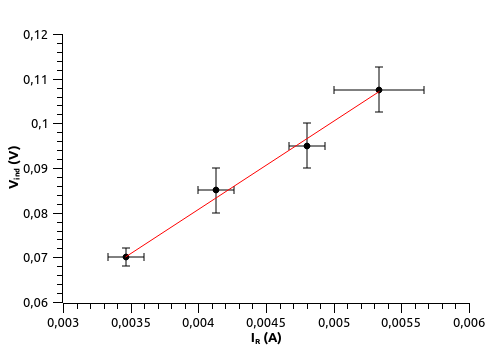
\includegraphics[width=0.9\linewidth]{grafica1}
	\caption{f = 1000 Hz}
\end{figure}

Ajuste: $ y = 19.7873x+ 0,0015$


%B=0.00151063079992389
%A=19.7873840009465
%A*x+B


\begin{figure}[H]
	\centering
	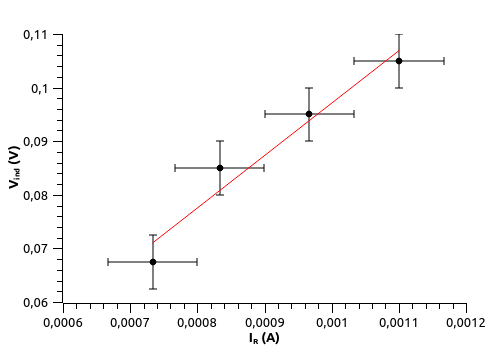
\includegraphics[width=0.9\linewidth]{grafica2}
	\caption{f = 5000 Hz}
\end{figure}

Ajuste: $ y = 97,909x - 0,0008$
%B=-0.000809090908964777
%A=97.909090908961
%A*x+B


\begin{figure}[H]
	\centering
	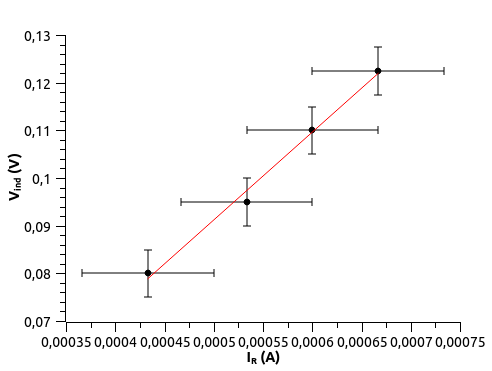
\includegraphics[width=0.9\linewidth]{grafica3}
	\caption{f = 7500 Hz}
\end{figure}

Ajuste: $ y = 184.346 x - 0,00105$

%B=-0.00105140186885627
%A=184.345794392009
%A*x+B


\vspace{\baselineskip}

\begin{table}[H]
	\centering
	\begin{tabular}{|lll|}
		\hline
		\multicolumn{1}{|c|}{f (Hz)} & \multicolumn{1}{l|}{C (F)} & K       \\ \hline
		1000                         & 19,79                  & 1,98   \\
		5000                         & 97,91                  & 1,98  \\
		7500                         & 184,37                 & 2,49 \\ \hline
		\multicolumn{3}{|c|}{$\bar{K}_{media} = 2,15$}                                \\ \hline
	\end{tabular}
	\caption{Valores de C y K obtenidos}
\end{table}


\subsection{Distribución del campo creado por una bobina}

Los resultados están representados en las Tablas 3, 4 y 5, medidos con una amplitud de 8V y una frecuencia de 5000 Hz.
Respectivamente, las Figuras 5, 6 y 7 representan gráficamente el campo frente a las coordenadas. Podemos ver que el campo solo depende de la distancia $z$.


\begin{table}[H]
	\centering
	\begin{tabular}{|c|c|c|}
		\hline
		$r$(m)$\pm0,001$ & $V_{ind}$(V)$\pm0,05$   & $B_o$ (T)                  \\ \hline
		0,02  & 0,095  & 0,0001 \\ \hline
		0,04  & 0,1    & 1,34E-05 \\ \hline
		0,06  & 0,105  & 3,97E-06 \\ \hline
		0,08  & 0,1125 & 1,68E-06 \\ \hline
		0,1   & 0,13   & 8,58E-07 \\ \hline
		0,12  & 0,16   & 4,96E-07 \\ \hline
		0,14  & 0,215  & 3,13E-07 \\ \hline
	\end{tabular}
	\caption{Campo en función del radio}
\end{table}


\begin{table}[H]
	\centering
	\begin{tabular}{|c|c|c|}
		\hline
		$\phi$ (º)$\pm0,1$ & $V_{ind}$(V)$\pm0,05$   & $B_o$ (T)                  \\ \hline
		45    & 0,285 & 2,094E-07 \\ \hline
		90    & 0,285 & 2,094E-07 \\ \hline
		135   & 0,28  & 2,094E-07 \\ \hline
		180   & 0,28  & 2,094E-07 \\ \hline
		225   & 0,285 & 2,094E-07 \\ \hline
		270   & 0,28  & 2,094E-07 \\ \hline
		315   & 0,29  & 2,094E-07 \\ \hline
		360   & 0,29  & 2,094E-07 \\ \hline
	\end{tabular}
	\caption{Campo en función del angulo}
\end{table}

\begin{table}[H]
	\centering
	\begin{tabular}{|c|c|c|}
		\hline
		$z$ (m) $\pm0,001$& $V_{ind}$(V)$\pm0,05$  & $B_o$ (T)                   \\ \hline
		0,05  & 0,19  & 2,37E-07 \\ \hline
		0,1   & 0,16  & 1,18E-07  \\ \hline
		0,15  & 0,12  & 7,90E-08 \\ \hline
		0,2   & 0,07  & 5,92E-08 \\ \hline
		0,25  & 0,05  & 4,74E-08 \\ \hline
		0,3   & 0,035 & 3,95E-08 \\ \hline
		0,35  & 0,012 & 3,38E-08 \\ \hline
		0,4   & 0,008 & 2,96E-08 \\ \hline
	\end{tabular}
	\caption{Campo en función de la distancia a la bobina}
\end{table}


\begin{figure}[H]
	\centering
	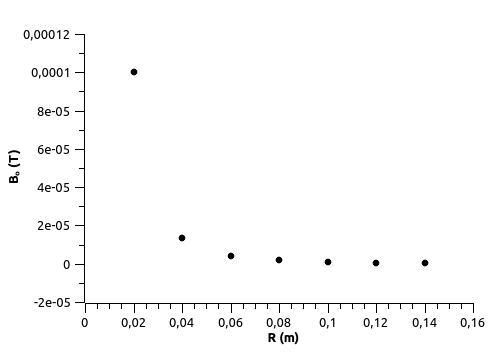
\includegraphics[width=0.9\linewidth]{grafica4}
	\caption{Campo en función del radio}
	\label{fig:grafica4}
\end{figure}
\begin{figure}[H]
	\centering
	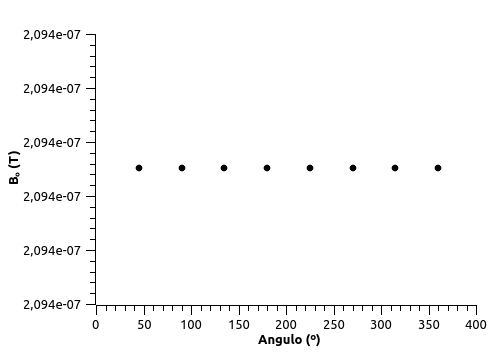
\includegraphics[width=0.9\linewidth]{grafica5}
	\caption{Campo en función del angulo}
	\label{fig:grafica5}
\end{figure}
\begin{figure}[H]
	\centering
	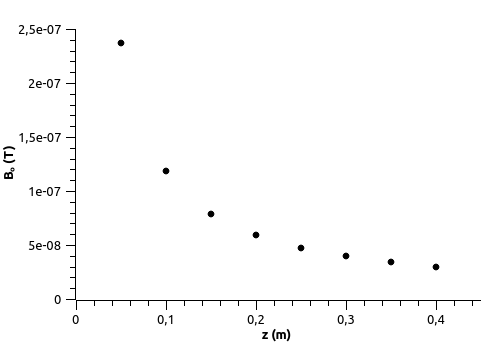
\includegraphics[width=0.9\linewidth]{grafica6}
	\caption{Campo en función de la distancia a la bobina}
	\label{fig:grafica6}
\end{figure}


\subsection{Distribución del campo creado por dos bobinas dispuestas coaxialmente. Bobinas de Helmholtz}

En la Tabla 6 vemos, para cuatro separaciones distintas de las bobinas, el voltaje inducido a lo largo de la distancia que las separa.



\begin{table}[H]
	\centering
	\begin{tabular}{|ll||ll||ll||ll|}
		\hline
		\multicolumn{2}{|l|}{d = 10 $\pm 0,1$ cm}      & \multicolumn{2}{l|}{d = 16 $\pm 0,1$ cm}      & \multicolumn{2}{l|}{d = 30 $\pm 0,1$ cm}      & \multicolumn{2}{l|}{d = 40 $\pm 0,1$ cm}      \\ \hline
		\multicolumn{1}{|l|}{z   (cm)} & $V_{ind} (\si{V})$  & \multicolumn{1}{l|}{z  (cm)} &$V_{ind} (\si{V})$  & \multicolumn{1}{l|}{z(cm)} & $V_{ind} (\si{V})$  & \multicolumn{1}{l|}{z (cm)} & $V_{ind} (\si{V})$ \\ \hline
		\multicolumn{1}{|l|}{1$\pm 0,1$}      & 0,064 & \multicolumn{1}{l|}{3$\pm 0,1$}      & 0,059 & \multicolumn{1}{l|}{5$\pm 0,1$}      & 0,044 & \multicolumn{1}{l|}{7$\pm 0,1$}      & 0,038 \\
		\multicolumn{1}{|l|}{3$\pm 0,1$}      & 0,066 & \multicolumn{1}{l|}{6$\pm 0,1$}      & 0,059 & \multicolumn{1}{l|}{10$\pm 0,1$}     & 0,036 & \multicolumn{1}{l|}{14$\pm 0,1$}     & 0,027 \\
		\multicolumn{1}{|l|}{5$\pm 0,1$}      & 0,066 & \multicolumn{1}{l|}{9$\pm 0,1$}      & 0,059 & \multicolumn{1}{l|}{15$\pm 0,1$}     & 0,034 & \multicolumn{1}{l|}{21$\pm 0,1$}     & 0,022 \\
		\multicolumn{1}{|l|}{7$\pm 0,1$}      & 0,066 & \multicolumn{1}{l|}{12$\pm 0,1$}     & 0,059 & \multicolumn{1}{l|}{20$\pm 0,1$}     & 0,036 & \multicolumn{1}{l|}{28$\pm 0,1$}     & 0,027 \\
		\multicolumn{1}{|l|}{9$\pm 0,1$}      & 0,065 & \multicolumn{1}{l|}{15$\pm 0,1$}     & 0,059 & \multicolumn{1}{l|}{25$\pm 0,1$}     & 0,044 & \multicolumn{1}{l|}{35$\pm 0,1$}     & 0,041 \\ \hline
	\end{tabular}
	\caption{Tensión inducida entre dos bobinas según la distancia a una de ellas}
\end{table}



%%%%%%%%%%%%%%%%%%%%%%%%%%%
\begin{thebibliography}{3}
%%%%%%%%%%%%%%%%%%%%%%%%%%%
	
	
	\bibitem{UNED2022} (varios) Guiones de prácticas- Técnicas Experimentales II. Grado en Física. Versión 2.1  UNED, 2022 \url{https://2022.cursosvirtuales.uned.es/o/3754218}
%	\bibitem{UNED2021} (varios) Técnicas Experimentales I. Versión 3.5.  UNED, 2021 \url{https://2021.cursosvirtuales.uned.es/o/42035617}
	%\bibitem{2021} Densidad de materiales \url{ https://www.stemm.com/index.php/es/densidades-de-materiales }
	
	
\end{thebibliography}


\end{document}
